\documentclass[12pt]{article}

\usepackage[top=1in,bottom=1in,left=1in,right=1in]{geometry}
\usepackage{amsmath,amssymb,mathtools}
\usepackage{xcolor}
\usepackage{graphicx}
\usepackage{hyperref}

\hypersetup{
    pdfauthor={},
    pdftitle={MATH 1075 - Lesson 6.1 Recitation}
}

\begin{document}

\vspace*{0.5in}

\begin{center}
    {\LARGE MATH 1075 - Section 7.7 Worksheet}

    \vspace{2em}

    {\large 09/29/2026}
\end{center}
\section{Review}
Solve following rational equation.
\vspace{1.5em}

1. $\frac{7b-4}{5b}=\frac{9}{5}-\frac{4}{b}   $

\vspace{4.5em}

2. $\frac{2}{4n-4}-\frac{7}{4}=\frac{-3}{n-1}    $

\section{Solving Proportions}
Solve following proportions.
\vspace{1.5em}

1. $\frac{6}{7}=\frac{96}{y}  $

\vspace{4.5em}

2. $\frac{15}{135}=\frac{w}{9}    $

\newpage

\section{Similar Triangle Problems}
\vspace{1.5em}


1. Triangle $XYZ $ is similar to triangle $ABC,$ solve for $x, y.$ 

\begin{figure}[htbp]
    \centering
    % Replace "my_image" with your actual file name (without extension)
    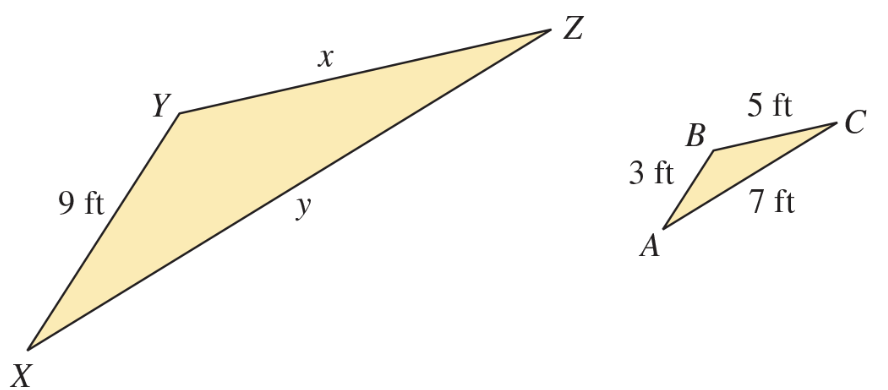
\includegraphics[width=0.8\linewidth]{similar triangle.png} 
\end{figure}

\vspace{10em}

\noindent 2. A 6-ft-tall man standing 54 ft from a light post casts an 18-ft shadow. What is the height of the light post?

\begin{figure}[htbp]
    \centering
    % Replace "my_image" with your actual file name (without extension)
    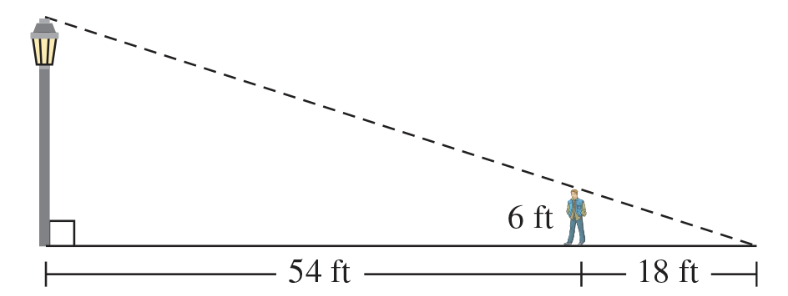
\includegraphics[width=0.8\linewidth]{street light.png} 
    \label{fig:my_figure}
\end{figure}
\newpage
\section{Distance, Time, and Rate Problems}

\vspace{1.5em}

1. A plane flies 630 mi with the wind in the same amount of time that it takes to fly 455 mi against the wind. If this plane flies at the rate of 217 mph in still air, what is the speed of the wind?
\vspace{12em}

\noindent 2. Devon can cross-country ski 5 km/hr faster than his sister Shanelle. Devon skis 45 km in the same amount of time Shanelle skis 30 km. Find their speeds.

\vspace{12em}
\noindent 3. Janine bikes 3 mph faster than her sister, Jessica. Janine can ride 36 mi in 1 hr less time than Jessica can ride the same distance. Find each of their speeds.

\vspace{12em}
\noindent 4. Amber jogs 10 km in $\frac{3}{4} $ hr less time than she can walk the same distance. If her walking rate is 3 km/hr less than her jogging rate, find her rates jogging and walking (in km/hr).

\vspace{12em}
\section{Work Application Problems}
\vspace{1.5em}
\noindent 1. The CUT-IT-OUT lawn mowing company consists of two people: Tina and Bill. If Tina cuts a lawn by herself, she can do it in 4 hr. If Bill cuts the same lawn himself, it takes him an hour longer than Tina. How long would it take them if they worked together?

\vspace{12em}

\noindent 2. A pipe can fill a reservoir in 16 hr. A drainage pipe can drain the reservoir in 24 hr. How long would it take to fill the reservoir if the drainage pipe were left open by mistake? (Hint: The rate at which water drains should be
negative.)

\end{document}
